%=========================================================================================================================================
%=========================================================================================================================================
\chapter{Background} \label{chapter:Background}
%=========================================================================================================================================
%=========================================================================================================================================



%-----------------------------------------------------------------------------------------------------------------------------------------
\section{Named Data Networking}
%-----------------------------------------------------------------------------------------------------------------------------------------

%-----------------------------------------------------------------------------------------------------------------------------------------
\subsection{NDN Fundamentals}
%-----------------------------------------------------------------------------------------------------------------------------------------

%hourglass architecture + figure \\
%interest \& data packets + figure \\
%router components and workflow (PIT, FIB, CS) + figure \\

 In NDN communication is driven by the receivers through exchanging two types of packets: \textbf{Interest} and \textbf{Data}. If a consumer wants to receive a chunk of data, he sends out an Interest into the network, which contains the name of the resource that should be acquired. The routers then forward the Interest until it ends up at the producer of said resource. The producer then deletes the Interest and in turn sends out a Data packet, containing the requested content, its name, and a signature from the producer's key (Figure \ref{fig:fundamentals:NDNPackagestructure}). 
 
 \begin{figure}[ht]
 	\centering
 	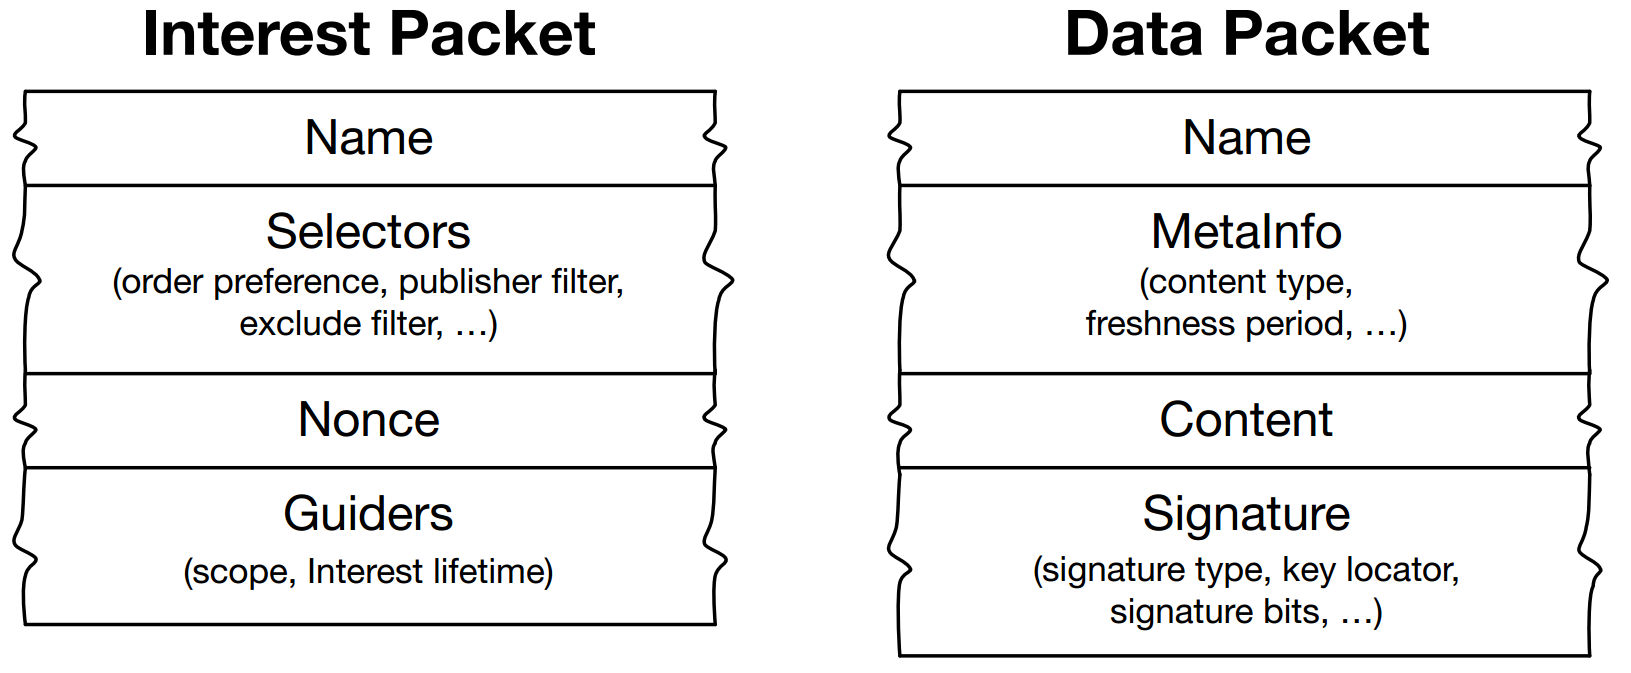
\includegraphics[width=0.8\textwidth]{figures/Packets_in_the_NDN_Architecture.png}
 	\figcaption{\textit{"Packets in the NDN Architecture."} \cite{ZABJ14}}
 	\label{fig:fundamentals:NDNPackagestructure}
 \end{figure}
 
 The Data packet travels back to the consumer, following the reversed path of the Interest that requested it. If the consumer wants further data, he has to send a new Interest. In order for this to work, all NDN routers are equipped with following data structures: A \textbf{Pending Interest Table (PIT)}, a \textbf{Forwarding Information Base (FIB)} and a \textbf{Content Store (CS)}. The PIT is a list containing entries for all Interests that have been forwarded, but not yet satisfied with a Data packet. The FIB has a routing protocol based on name-prefixes and decides where to forward Interests when applicable, following a specific forwarding strategy. The CS is a temporary cache for all the Data packets that recently satisfied Interests. Since an NDN Data packet is meaningful independent from source or destination, it can be distributed by the router itself if the same Data is requested by multiple consumers within a short period. Using all these data structures, the forwarding process at an NDN router looks as follows (see also Figure \ref{fig:fundamentals:NDNForwardingProcess}):
 
 \begin{figure}[ht]
 	\centering
 	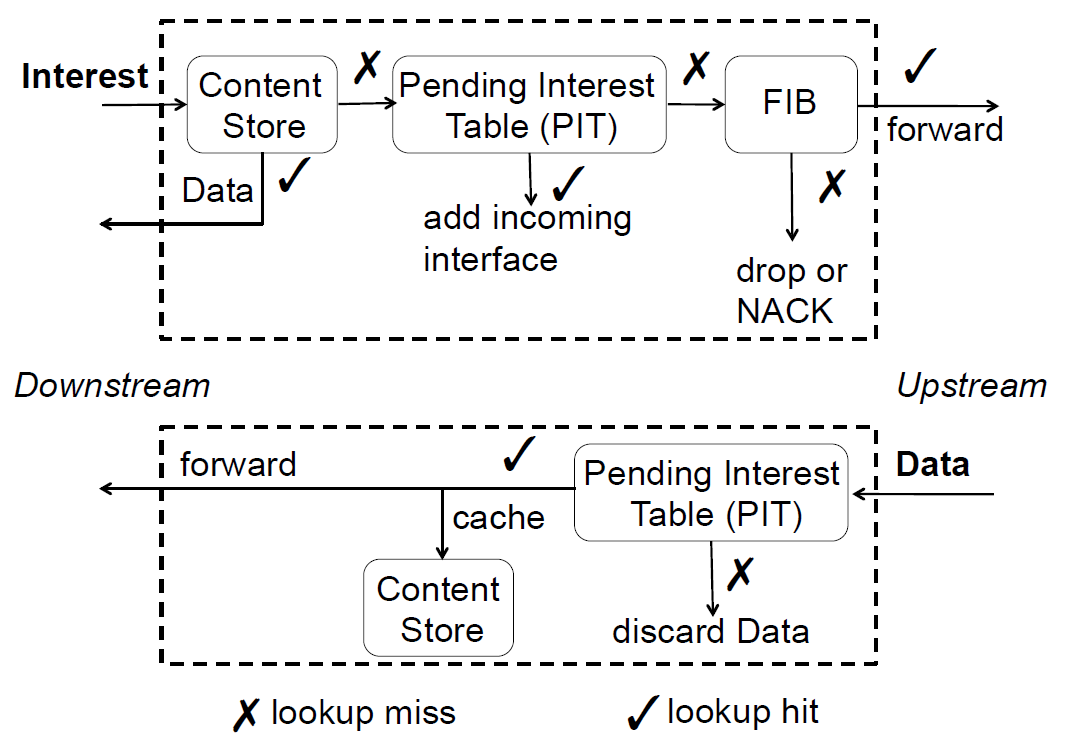
\includegraphics[width=0.8\textwidth]{figures/Forwarding_process_at_NDN_Router.png}
 	\figcaption{\textit{"Forwarding Process at an NDN Node."} \cite{ZABJ14}}
 	\label{fig:fundamentals:NDNForwardingProcess}
 \end{figure}
 
 
 When an Interest arrives at the router, the first thing it does is to look if the requested data is already available in the CS. If so, the Interest can be satisfied immediately and the corresponding Data packet is sent back. Otherwise, the router checks if the name contained in the Interest is already saved as an entry in the PIT. If it is, someone else has requested the same data but it has not yet arrived. If that is the case, the incoming interface will be added to the PIT entry. If there is no entry yet, a new entry is created and the packet will be forwarded to a node closer to a possible source, which is determined by the FIB via a name-prefix based protocol. If a Data packet arrives at an NDN Router, the PIT is searched for a matching entry. If no entry is found, the data packet will be discarded. Otherwise, the Data packet is then duplicated and send to each downstream interface noted there, followed by the removal of said entry from the PIT. The Data is then saved in the CS in case it will be requested again in the near future. This whole process ensures that "routing" is only needed towards the producer of content since the Data packets simply follow the reversed path of their corresponding Interest. It also ensures that the number of Interest and Data packets stay the same (given that no packets are lost), creating a \textbf{flow balance}, similar to what TCP provides. The key difference here is that TCP was built as an additional layer over IP, while in NDN the flow balance is an in-built feature. In fact, no additional transport layer is required at all, because NDN takes on many of its tasks by itself anyway. The rest (like de-multiplexing, reliable delivery, etc.) will be managed by the applications themselves if they actually require those features. \cite{ZABJ14}


%-----------------------------------------------------------------------------------------------------------------------------------------
\subsection{NDN Specifics}
%-----------------------------------------------------------------------------------------------------------------------------------------
The following section aims to discuss specific aspects of NDN in further detail. %TODO is this even necessary?

%-----------------------------------------------------------------------------------------------------------------------------------------
\subsubsection{Naming}
%-----------------------------------------------------------------------------------------------------------------------------------------
%Structure of name
%it's hierarchical --> allows scaling
%names/routing unique only within its scope (smart home - global)

%dynamically generated contnt needs names to be constructed deterministically (algorithm, rule)
%partial names + selecter like "leftmost child" also possible

%its' opaque to the network --> independently developed by each app
%freedom for developers/apps to shape naming to their needs
%guidelines and libraries to facilitate naming conventions though

One of the biggest and most characteristic features of NDN is the naming itself. A name in NDN can be used to reference a multitude of things, from a simple command to whole chunks of a video. An example of the latter could look like \textit{"/itec/videos/demo.mp4"}. While not completely necessary, most names in NDN have some sort of hierarchical structure, with different levels separated by a "/", not unlike current URLs. This allows for much easier scaling than flat names, especially considering that namespaces for data that should be available worldwide need unique names on a global scale. There are however also use cases like smart homes where the requirements for uniqueness are significantly smaller and can be used to map dependencies and relations like in \textit{"/myhome/bedroom/lights/off"}.

In order to request data, the name must first be known to the consumer. While this may be feasible with static content, dynamic content needs names to be constructible deterministically by both consumer and producer. This can be achieved by using algorithms or rules that are known and agreed upon by both parties. Alternatively, Interest selectors in conjunction with longest prefix matching can be used to request data without knowing the full naming structure. For example, the first section of a video might be requested with \textit{"/itec/videos/demo.mp4/"} and the \textit{"leftmost-child"} selector, which the producer could then answer with sending \textit{"/itec/videos/demo.mp4/1/"}.

Despite this breadth of possibilities in naming, the routers do not actually know most of its meaning, which makes the name \textbf{opaque} to the network. This allows the network and application layer to be developed independently from each other and gives developers the freedom to shape naming to the needs of their application. Nevertheless, there are efforts to streamline this process by providing libraries and guidelines to facilitate naming conventions to some degree. \cite{ZABJ14,ZEBJ10}
%-----------------------------------------------------------------------------------------------------------------------------------------
\subsubsection{Forwarding}
%-----------------------------------------------------------------------------------------------------------------------------------------
%no address exhaustion
%no address management
%can use existing *routing* algorithms
%announce name prefixes of data you serve, which then get distributed to other routers FIB
%conventional routing protocols can be adapted (OSPF/BGP)
%individual PIT state per router (per-hop/per-packet)
%adaptive forwarding strategy module (unsatisfied Interest capacity, priority, load balancing)
%.NACK (if upstream is down, congestion, etc.) --> maybe alternate path from receiving router?
%natural multicast support (PIT entries)
%regulate number of pending interests to regulate traffic load (due to flow balance)

A router in NDN announces name prefixes (similar to current IP prefixes) of the data it is willing to serve, which then get distributed to other router's FIBs. By making small adaptions, many of the current algorithms (e.g. links-state and distance vector) and protocols (e.g. OSPF and BGP) can still be used in NDN. Additionally, having no IP addresses and a theoretically unbounded namespace eliminates problems plaguing the current Internet like address space exhaustion, NAT traversal, or address management. 

Each router in NDN manages its own PIT, adding entries for incoming Interests and removing them after they have been satisfied with corresponding Data packets or after a timeout. In case of congestion or upstream link failure, a NACK can be sent to downstream neighbors, which can in turn decide to try alternative paths. For this purpose, each router contains a \textbf{forwarding strategy module}, which makes informed decisions about which Interests are forwarded where, unsatisfied Interest list capacity, the priority of different Interests, and load balancing. The latter can be achieved due to NDNs inherent flow balance. Since each Data packet needs its own Interest, by regulating the rate of forwarding pending Interests NDN routers can effectively regulate traffic load.

Additionally, aggregating entries of incoming Interests for the same Data packet in the PIT allows for natural multicast support, since an incoming Data packet will be forwarded to all downstream neighbors who showed interest. \cite{ZABJ14}
%-----------------------------------------------------------------------------------------------------------------------------------------
\subsubsection{Caching}
%-----------------------------------------------------------------------------------------------------------------------------------------
%packets independently meaningful (name + signature)
%data chached in content store--> satisfy future requests for the same data
%origin of data (cache or source) is not differentiated
%dynamic content benefits if multicast or for retransmission after error
%repostory instead of todays CDNs (in-network solution, no need for app layer overlay)
%privacy IP: addresses + payload (who consumers what)
%privacy NDN: names (what is consumed, but harder to know by whom)

In NDN each Data packet carries a name and signature, making it independently meaningful and identifiable, no matter where it is found in the network. This allows each router along the path to cache packets in their content store, potentially decreasing traffic load and response times if others request the same Data in the near future. Whether the packet ultimately comes from a cache or the source is not differentiated in NDN. While this benefits static files the most, it should be noted that dynamic content can also benefit from in-network caching in case of multicast being used, or if retransmissions are required after a package loss. 

In addition to each router's CS, NDN networks can also provide so-called \textbf{Repositories (REPO)}. These caches can save much larger volumes of data and keep it persistent for longer periods. The idea is to offer in-network solutions for today's CDNs, instead of using workarounds with application layer overlays.

Even though Data packets might raise certain security concerns, the specifics are different from IP architectures. Where in current solutions an attacker might see addresses and the payload, NDN packets only have names. While it might be easier to see what is being consumed, the lack of addresses makes it way harder to identify by whom in most cases. \cite{ZABJ14}

%-----
%
%Data packets in NDN are identified by name and signature and are therefore valid and meaningful independent from source or destination. This allows them to be cached in a routers CS for later requests, while not making a difference between storage or network channels. For static files NDN can achieve near optimal data delivery, but even dynamic files benefit from in-network caching by using multicast or for retransmission after a packet loss. 
%
%%NDN also supports for larger and more persistent in-network storage options called \textbf{Repositories (REPO)}. They could potentially supersede today's Content Delivery Networks (CDN) by offering the same services without the need to involve application layer or use special protocol tricks. 
%
%Caching in NDN does however raise some privacy concerns. While in IP architecture the source and destination of a datagram (and possibly its payload as well) were visible throughout the network, in NDN the name is open for read by every node. Although this may allow outsiders to view which data is requested, it is way harder to link it to a consumer, since there are no destinations in an NDN datagram. Nevertheless, in-network caching remains one of the strongest features NDN has to offer.

%-----------------------------------------------------------------------------------------------------------------------------------------
\subsubsection{Security}
%-----------------------------------------------------------------------------------------------------------------------------------------
In contrast to TCP/IP, which treated security as an afterthought, one of NDN's architectural principles was to include security as an in-built feature from the get-go. \cite{ZEBJ10} Instead of armoring channels to prevent attacks, NDN focuses on data-centric security. More specifically, that means that every Data packet is required to be cryptographically signed. This decouples the consumer's trust from how and where data is obtained and instead shifts the attention to the validity and possible harmfulness of the packet itself. It also means that NDN has inherent resistances against spoofing and tampering, while its architecture and forwarding procedure make it harder to use prefix hijacking since anomalies caused by attacks can be detected and data be retrieved from alternative paths. 

Furthermore, the absence of destination addresses makes it difficult to target attacks to specific devices. Additionally, PIT timeouts can offer relatively cheap attack detection. Unfortunately, NDN also comes with new attack possibilities and vulnerabilities, like DoS through Interest flooding, although the effect of this type of attack can be limited by constraining the size of the PIT. \cite{ZABJ14}
%-----------------------------------------------------------------------------------------------------------------------------------------
\subsubsection{Mobility} \label{subsubsection:Mobility}
%-----------------------------------------------------------------------------------------------------------------------------------------
Mobile nodes become more and more important and - like many other things - are just solved as a patch to the original system in TCP/IP. Despite not being the main focus point in NDN either, there are at least thoughts on how it could work within the architecture. When a subscriber moves in NDN after sending an Interest, he can just send a new Interests after moving and re-request everything he has not yet received, since the additional Interests will be suppressed at the first node both routes have in common anyway. The Data packet will however be transported to the old and new location alike. 

Moving publishers is a much more difficult problem though because after moving the producer has to newly advertise the name prefixes for the information he is hosting so that all routers with FIB entries pointing to the publisher can be updated. In high mobility scenarios, this can produce a large amount of overhead, although it can be partially mitigated by using the Listen First Broadcast Later (LFBL) protocol. LFBL floods the network with interests until a data source is found. The source then listens if any other sources already sent a matching data packet and then proceeds to send one itself if it does not hear of any others. \cite{ZABJ14}
%-----------------------------------------------------------------------------------------------------------------------------------------
\subsection{NDN Limitations}
%-----------------------------------------------------------------------------------------------------------------------------------------
%Current obstacles and problems? \\
%Current open questions in science?


Despite being a quite promising architecture, NDN is far from being flawless or complete. Several areas and topics are either not yet researched enough or not tackled at all. The following is a collection of current limitations and shortcomings of NDN:

\begin{itemize}
	
	\item NDN is trending towards a hierarchical name structure, but there is no clear consensus in the community yet, whether flat names or hierarchical ones are better-suited \cite{XVSF+13}. Hierarchical names can be human-readable and are easier to aggregate, but it is unclear if they are scalable enough for worldwide deployment. Flat names on the other hand are easier to administer and are highly scalable with Distributed Hash Tables (DHTs) but it is unclear if DHTs offer needed performance. Additionally, there are also little to no solutions yet regarding versioning, deletion, and revocation of names. In TCP/IP this was of little concern to the network layer, but in NDN, where everything is based on the names of data, this is no easy task. In fact, it is not even clear yet at what granularity names should be given. A named object could correspond to a packet, variable-sized information chunks, or entire application-level objects \cite{XVSF+13}. What is clear though, is that there is still a long road of research ahead regarding naming in NDN.
	
	\item While much thought has been spent on solutions for intra-domain routing in NDN, inter-domain routing has not yet received much attention. In fact, this is topic is not even fully fleshed out for current internet architecture \cite{XVSF+13}. On one hand, inter-domain routing is strongly affected by business relationships between the involved parties, on the other hand, there are also noticeable limitations when trying to scale the architecture to worldwide sizes. 
	
	\item As already mentioned in section \ref{subsubsection:Mobility}, publisher mobility is still a major challenge in NDN, due to a large amount of overhead introduced by having to re-advertise after moving and the fact that NDN's name resolution is relatively slow to update.
	
	\item Even though in-built security is one of the main architectural principles of NDN, it is still based on cryptographic keys. While several approaches could be (and partially have been) investigated, there are no clear solutions yet concerning distribution, managing, and revocation of said keys. Additionally, even though the nature of NDN's architecture and workflow offers inherent resistances against many of today's attacks, there are also new, NDN-specific ways to violate privacy. Since the names of requested objects are visible on every router, a new form of protection has to be found to mitigate potentially unwanted observations of outsiders.
	
	\item Due to the nature of NDN, the network layer may potentially gain many new mechanisms and functionalities to enhance productivity. Features like in-network caching, multicast, and multi-path routing also affect the transport layer, requiring a huge redesign. The problem here is though, that NDN is still under active development, so the amount of research that can be done regarding the transport layer is quite limited but will have to be tackled in the future.
	
	\item NDN is by design an inherently pull-based architecture. This makes it rather difficult to use for applications and use cases with a push-based nature, like conversational services, video streaming, and live content. By default, every bit of video data has to be requested by the user due to flow balance, increasing the number of Interests and therefore packets by a significant amount, straining the network in the process. Furthermore, if a consumer wants to receive live content on time, he would theoretically have to send Interests for Data before it has been produced. This either requires the ability to predict the future or a well thought out strategy and naming scheme on the producer side, which in turn has to be known by the consumer.
	
	
	
\end{itemize}

Besides all the technical limitations and open questions mentioned above, there are also business and logistical obstacles to overcome. Worldwide deployment of NDN would most certainly have to be incremental. While an overlay solution might be relatively easy, only a full native deployment (a "clean-slate" solution) can offer all the expected improvements. Furthermore, even under the assumption, everything might be technically possible, there are still unanswered questions left like: Which application areas should it be deployed to first? What happens to current CDNs, since they will probably become mostly redundant. How should Internet providers adapt their business models? All of these questions (and many more!) need to be answered before NDN is ready for the world. 
\cite{XVSF+13}


%-----------------------------------------------------------------------------------------------------------------------------------------
\section{Adaptive Video Streaming}
%-----------------------------------------------------------------------------------------------------------------------------------------
Nowadays we find ourselves confronted with an ever-growing demand for video streaming. Video-chats, live-streams, and video on demand make up a significant fraction of today's Internet traffic. Tackling such quantities of data requires efficient handling to keep up with the increasing requirements. Furthermore, static solutions do not offer the needed performance, since network conditions can vary for every consumer and are always prone to change, requiring more adaptive solutions. While there are several approaches to solve this problem, this section focuses on the advancement of adaptive rate control in particular. 

%-----------------------------------------------------------------------------------------------------------------------------------------
\subsection{Adaptive Rate Control}
%-----------------------------------------------------------------------------------------------------------------------------------------
This approach focuses on the adaption of a video's bitrate to fit the current requirements and possibilities, dictated by the network capabilities at a given moment in time. One consumer-driven approach to do so is by splitting the video into several parts on the producer side \cite{MQGW12}. Then each part is encoded in several representations or bit rates, each representing a different level of quality. The consumer can subsequently decide which quality he wants and start requesting video parts of said level. If the network parameters change and require a switch in quality to keep the stream up, the consumer can select different representations for the following parts to better fit the new network environment.

It should be noted that with this approach the consumer is responsible for analyzing the current network conditions and deciding which level of quality best suits the given situation. This can be done by estimating available future throughput by measuring the current one and making predictions. Additionally, the video buffer on the consumer side can be an indication when to switch to a different representation. A near-empty buffer suggests switching to a lower bitrate, while a full one indicates that higher bit rates might be possible. \cite{MQGW12}

While these approaches can lead to very precise adaption to the network situation at hand, one must not forget the human behind the screen who watches the content. Switching content quality every second or buffering for half a minute before the video plays might be exactly what the network demands, but will probably still be detrimental for the user experience. Thus, a careful balance has to be found, requiring the application to juggle network capabilities and switching restrictions, all while keeping start-up delay to a minimum.

%-----------------------------------------------------------------------------------------------------------------------------------------
\subsection{Dynamic Adaptive Streaming over HTTP (DASH)}
%-----------------------------------------------------------------------------------------------------------------------------------------
%%ISO/IEC, Information Technology: Dynamic Adaptive Streaming Over
%%HTTP (DASH) Part 1: Media Presentation Description and Segment
%Formats, Standard ISO/IEC 23009-1:2012, 2012. [Online]. Available:
%https://www.iso.org/iso/iso_catalogue/catalogue_tc/catalogue_
%detail.htm?csnumber=57623

%TODO this whole paragraph could probably be cut if needed.
Normally when writing applications, one would trust the transport layer to minimize induced delays and deliver data with an appropriate degree of reliability and timeliness \cite{KuAB17}. However, with how tight some time requirements are when it comes to live-streaming and some multimedia content delivery in general, those mechanisms used by TCP \cite{Poot81} might actually be a hindrance. It might better to just skip a frame that did not manage to arrive in time than to invest network resources to make sure it gets re-sent, either blocking further frames from playing or being useless on arrival since the video already went on. This is the reason why early approaches focused on using UDP \cite{Poot80} since it offered a simple base for transport without the extra baggage. Unfortunately, this approach encountered problems with firewalls and other deployment issues, which eventually resulted in the TCP based HTTP \cite{BePT15} to become the more popular choice for multimedia delivery, since it works out of the box and is let through most firewalls by default.  

% \begin{figure}[ht]
% 	\centering
% 	\includegraphics[width=0.8\textwidth]{figures/DASH_MPD_structure_example.png}
% 	\figcaption{The Multimedia Presentation Description hierarchical data model. In this example, MPD contains three periods, period 2 contains three adaptation sets and the adaptation set 1 contains four representations, including three representations with various bit rates and one representation for trick mode. Finally, representation 2 consists of its segment info, which consequently includes its initialization segment and four media segments' information. \cite{Soda11}}
% 	\label{fig:fundamentals:DASH_MPD_structure}
% \end{figure}
 
  \begin{figure}[ht]
  	\centering
  	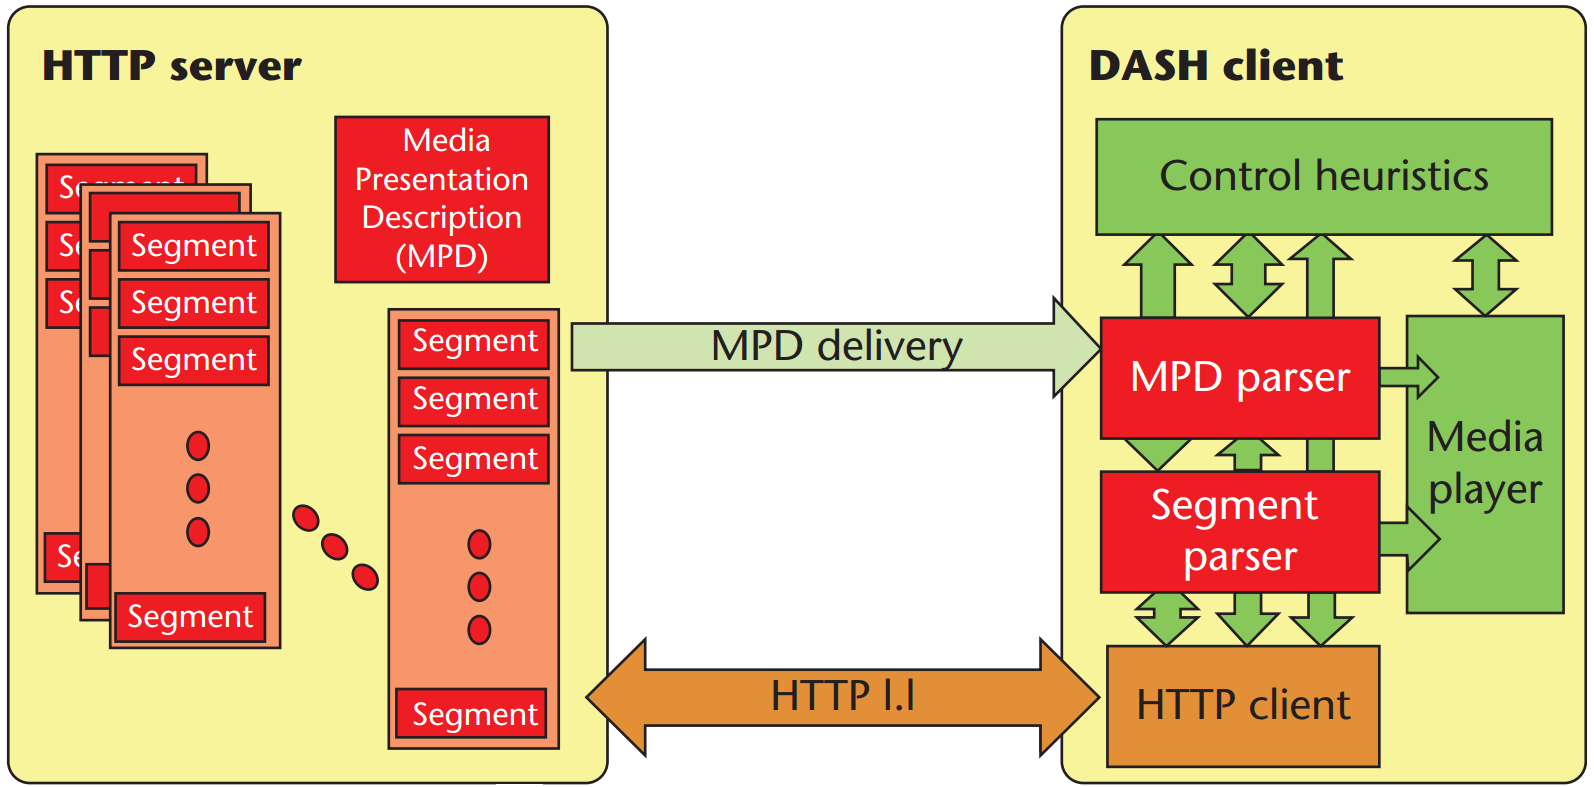
\includegraphics[width=0.8\textwidth]{figures/DASH_scope.png}
  	\figcaption{\textit{"Scope of the MPEG-DASH standard. The formats and functionalities of the red blocks are defined by the specification. The clients control heuristics and media players, which aren't within the standard's scope."} \cite{Soda11}}
  	\label{fig:dash:DASH_scope}
  \end{figure}

Thus the current standard for multimedia consumption is \textbf{MPEG-DASH} \cite{Soda11}. It specifies a format in which the segments for different representations are stored on a server, ready to be downloaded on demand. To do so, the customer first requests a so-called \textbf{Media Presentation Description (MPD)}. This file contains information about which quality variations are available, their exact parameters and specifications, how frequently they can be switched, in which order they are meant to be consumed, and finally the direct links to download corresponding segments. After that, it falls to the client's responsibility to pick the appropriate segment for the time, requirements, and current network capabilities. Note that only segments, MPD and their respective parsers (see red sections in \ref{fig:dash:DASH_scope}) are defined by the standard, leaving the other components open to competition and individual adaption.

%how it works:
%producer has video split up into parts, each available in multiple representations or quality levels
%consumer requests MPD (Media Presentation Description) file 
%	--> gets info on all available representations and how to request them (naming schemes/addresses)
%starts requesting first part of video in high quality
%can change to another quality after every segment (every few seconds)
%\cite{Soda11} (DASH src paper)

%-----------------------------------------------------------------------------------------------------------------------------------------
\subsection{Adaption logics}
%-----------------------------------------------------------------------------------------------------------------------------------------
While splitting multimedia data into segments of different quality levels is a necessary foundation for Adaptive Rate Control, the real challenge lies within selecting the right segment at the appropriate time, based on current network conditions and capabilities. This is done by a so-called \textbf{Adaption Logic}, an algorithm or collection of software mechanisms that handle the decision making behind ARC and can make or break the concept of adaptive streaming. A good adaption logic might strive to answer the following questions: 

\begin{itemize}
	
	\item How do I measure the current network status, to extract meaningful information that can be used as a base for the other decisions? 
	
	\item Can or should I try to predict changes in network status for the near future? 
	
	\item Under what circumstances do I switch to another representation? 
	
	\item If I decide to select another set of sections, what quality level do I go for, and how big are my steps to get there? 
	
	\item How long should I wait before actually switching to another quality? 
	
	\item How often am I allowed to switch in a given interval?
	
\end{itemize}

There are a lot of adaption logics out there that try to answer these questions. The following sections will describe some of them in greater detail, based on the works of \cite{TiMR16}.

%-----------------------------------------------------------------------------------------------------------------------------------------
\subsubsection{DASH-JS} 
%-----------------------------------------------------------------------------------------------------------------------------------------

DASH-JS \cite{RLMT12} uses bandwidth estimation based on previous downloads to predict what the future bandwidth might be and chooses a quality for the next segment accordingly. It does so by using a simple equation shown in \ref{equation:adaptionLogics:DASH-JS}, where $b_{n}$ stands for the estimated bandwidth of the next segment that needs to be downloaded.

\begin{equation}
b_{n} = \dfrac{w_{1}b_{n-1} + w_{2}b_{m}}{w_{1}+w_{2}}
\label{equation:adaptionLogics:DASH-JS}
\end{equation}

The next segment's bandwidth is calculated by looking at the calculation of the last segment's bandwidth $b_{n-1}$ and the actual measured bandwidth of said segment $b_{m}$. Those values are given different priority with weights $w_{1}$ and $w_{2}$, which default to $w_{1}=0.7$ and $w_{2}=1.3$ according to \cite{RLMT12} if nothing else is specified. Thus the bandwidth for the next segment is calculated by taking the last calculation as a base and adjusting it based on the actual measurements, bringing the previous prediction in line with reality to form a new one. The algorithm then looks at the range of available representations and chooses the one with the highest quality that can still be sustained at the currently estimated bandwidth. The initialization of this whole process uses the measured bandwidth of the MPD file download as a base.
%-----------------------------------------------------------------------------------------------------------------------------------------
\subsubsection{Miller et al.}
%-----------------------------------------------------------------------------------------------------------------------------------------
The algorithm presented by Miller et al. \cite{MQGW12b} belongs in the category of buffer based adaption logics and works in two phases. During the startup phase, it tries to increase quality rather aggressively, to reach an appropriate representation faster. It then transits into the stable phase, where the focus lies on maintaining a healthy level of buffered multimedia material. In order to accomplish this, the adaption logic defines a set of thresholds $0 < b_{min} < b_{low} < b_{max}$ where $b$ denotes the current fill level of the buffer. The algorithm aims to keep said fill level around an optimum defined as $b_{opt}= 0.5(b_{low}+b_{max})$. It does so by taking the current buffer level and the last segment's throughput as input, recommending a switch to a lower quality if the buffer gets too low or to a higher representation if the buffer is substantially fuller than needed. The overlying guidelines for these decisions are to maximize the played bitrate while minimizing the number of quality switches for the user.


%buffer level and last throughput as input
%recommended bitrate and minimum buffer level for download as output
%maximize bit rate, minimize quality switches
%two phases: startup - agrressive increase of quality
%stable phase - maintain healthy buffer level
%defines thresholds: $(0 < b_{min} < b_{low} < b_{max})$ 
%optimal buffer level: $b_{opt}= 0.5(b_{low}+b_{max})$.
%
%Describe Miller et al. \cite{MQGW12b}

%-----------------------------------------------------------------------------------------------------------------------------------------
\subsubsection{Thang et al.}
%-----------------------------------------------------------------------------------------------------------------------------------------
Thang et al. \cite{THKP12} published the idea for an adaption logic that looks further into the past than just the last segment. Each time a segment is received, the throughput is calculated and saved into a list. The algorithm then calculates the average of all the values in said list, creating a rough estimation of the throughput in the recent past. After enough values have filled the list for it to reach its maximum capacity, every new throughput measurement causes the oldest entry in the list to drop out. This ensures that the calculated average stays fresh and relevant. By basing the selection of an appropriate quality level on this average throughput, it allows the algorithm to achieve a smoother playback during short term bandwidth fluctuations since singular deviations do not have that much of an impact on an average calculated over a set of multiple numbers. Furthermore, the maximum list capacity ensures that drastic changes in bandwidth still have a noticeable impact, even as time goes on, allowing the adaption logic to quickly react and adapt if needed. 

%sliding average of measured video throughput
%dynamically adapts to changing bandwidth conditions
%smooth playback during short term bandwidth fluctuations
%quick reaction if strong bandwidth change

%Describe Thang et al. \cite{THKP12}

%what are those? \\
%which are interesting here? \\
%present a few. 
%how to decide:
%	how to measure network status?
%	how/if to predict changes in network status?
%	when to switch to another quality?
%	what to quality to switch to?
%	how fast to switch to that quality?
%	how often is switching allowed?
	

%-----------------------------------------------------------------------------------------------------------------------------------------
\section{Quality of Experience}
%-----------------------------------------------------------------------------------------------------------------------------------------
what is important for conversational services? \\
end-to-end latency, packet loss...

Low transmission delay
Low packet loss
Low jitter (what is that again?)

%-----------------------------------------------------------------------------------------------------------------------------------------
\subsection{Metrics} %TODO Maybe delete thos headline and elevate the metrics to subsections instead
%-----------------------------------------------------------------------------------------------------------------------------------------
can be objective or subjective --> only objective metrics here
work by comparing resulting image (after compression, transformation, transmission, etc) with original image
%-----------------------------------------------------------------------------------------------------------------------------------------
\subsubsection{Peak Signal to Noise Ratio (PSNR)}
%-----------------------------------------------------------------------------------------------------------------------------------------
pro: easy to use/calculate
con: only suitable if video content and codec do not change \cite{HuGh08}

\begin{equation}
PSNR (f,g) = 10 \cdot log_{10}\left(\dfrac{255^{2}}{MSR(f,g)}\right)
\label{equation:metrics:PSNR_1}
\end{equation}

\begin{equation}
MSR(f,g) = \dfrac{1}{MN}\sum_{i=1}^{M}\sum_{j=1}^{N}(f_{ij}-g_{ij})^{2}
\label{equation:metrics:PSNR_2}
\end{equation}

%-----------------------------------------------------------------------------------------------------------------------------------------
\subsubsection{Structural Similarity (SSIM)}
%-----------------------------------------------------------------------------------------------------------------------------------------


\begin{equation}
SSIM(f,g) = l(f,g) \cdot c(f,g) \cdot s(f,g)
\label{equation:metrics:SSIM_1}
\end{equation}

\begin{equation}
l(f,g) = \dfrac{2\mu_{f}\mu_{g}+C_{1}}{\mu_{f}^{2} + \mu_{g}^{2}+C_{1}}, 
c(f,g) = \dfrac{2\sigma_{f}\sigma_{g}+C_{2}}{\sigma_{f}^{2} + \sigma_{g}^{2}+C_{2}}, 
s(f,g) = \dfrac{\sigma_{fg}+C_{3}}{\sigma_{f}\sigma_{g}+C_{3}}
\label{equation:metrics:SSIM_2}
\end{equation}

%-----------------------------------------------------------------------------------------------------------------------------------------
\subsubsection{Video Multimethod Assessment Fusion (VMAF)}
%-----------------------------------------------------------------------------------------------------------------------------------------
pro: range of tests --> more complete picture
con: more difficult/time-y to use/calculate

%=========================================================================================================================================
%=========================================================================================================================================
% EOF
%=========================================================================================================================================
%=========================================================================================================================================
